\subsection{Retrieval of compound identity and mechanism of action}
Recognizing the same drug requires reproducible identity features, whereas connecting different drugs sharing an MOA requires functional similarity. A retrieval framework should preserve both relationships across morphology and expression. We evaluated same-drug identity in U2OS and A549 (Fig.~2A), then excluded query-drug matches to assess within- and cross-modal MOA retrieval (Fig.~2B), alongside local image neighborhoods (Fig.~2C).

\resultfigure{2}

The compound head identified the same drug across crops (Fig.~2A). U2OS Top-1 hit rates were 99.19\% for BioMoAX and 96.22\% for CellCLIP, both near the task ceiling. In A549, BioMoAX achieved 92.00\%, versus 72.23\% for CLOOME.

Excluding same-drug matches, BioMoAX retrieved other compounds sharing an MOA (Fig.~2B). CellCLIP had higher I2I means in both cell lines, but differences were not significant. BioMoAX matched raw L1000 in U2OS E2E at 22.22\% and exceeded it in A549 (20.60\% versus 17.94\%).

BioMoAX\textquotesingle s main advantage is cross-modal functional matching: connecting mechanism-related morphology and expression responses in a common MOA space enables reciprocal retrieval. This advantage is clearer in A549, where BioMoAX\textquotesingle s I2E Top-5 hit rate was 12.29\%, versus 8.11\% for ridge-mapped CellCLIP, and E2I was 16.94\%, versus 13.29\% for ridge-mapped CellProfiler, the strongest corresponding baselines.

In A549, BioMoAX and CellProfiler had similar I2I performance but different I2E hit rates (12.29\% and 6.31\%). CellCLIP had higher I2I means yet lower means in both cross-modal directions. These comparisons distinguish image-only mechanism discrimination from morphology--expression matching, consistent with directly learning functional correspondence. Relative to baselines, cross-modal gains are concentrated in A549 and cover both image-to-expression and expression-to-image retrieval.

Figure~2C compares local neighborhoods of the same highlighted crops across methods. In several BioMoAX neighborhoods, responses to different drugs sharing an MOA overlap, forming multi-compound functional neighborhoods. This complements retrieval with same-drug matches excluded: the framework retains drug identity and connects related responses across compounds in the MOA space, supporting queries between morphology and expression.

\subsection{Mechanism-related retrieval across experimental batches}
Experimental protocols and imaging conditions can shift representations across sources, obscuring functional similarities. We tested whether an existing library supports queries from another source, using cpg0030 images to query cpg0012. All 115 queries have other reference drugs sharing an MOA but no identical-compound matches, requiring matching across sources and compound identities (Fig.~3A).

\begin{figure}[!htb]
\centering
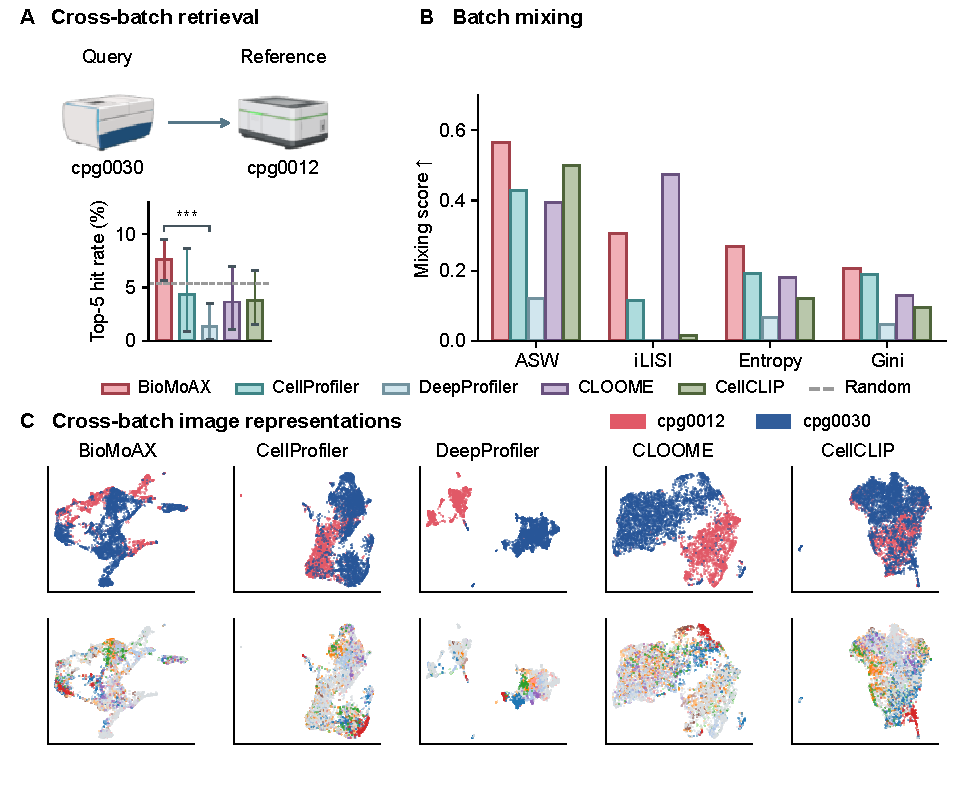
\includegraphics[width=\linewidth]{figures/fig3.pdf}
\caption{\csname captionFigure3\endcsname}\label{fig:3}
\end{figure}

Top-5 hit rates were 7.59\% for BioMoAX, 4.35\% for CellProfiler, 1.39\% for DeepProfiler, 3.65\% for CLOOME and 3.83\% for CellCLIP, with a 5.37\% random reference. BioMoAX had the highest mean; only its difference from DeepProfiler was significant after correction of paired Wilcoxon tests. Retrieved positives connect different compounds, showing that functional information remains retrievable across sources. Limited absolute hit rates leave substantial room for improvement.

For 32 shared compounds, mixing was assessed with drug identity held constant (Fig.~3B). In the displayed comparison, BioMoAX had the highest ASW, entropy and Gini scores; CLOOME had the highest iLISI. Crop-level maps show partial source overlap for BioMoAX, CellProfiler and CellCLIP, versus more pronounced separation for DeepProfiler (Fig.~3C). Mixing evaluates same-drug similarity across sources; MOA retrieval tests functional relationships between different drugs. Together, these analyses assess whether source-related separation can be reduced while preserving information that distinguishes and connects drug responses. The results support reusing existing measurements for mechanism-related queries from another experimental source.

\subsection{Mechanism-related retrieval across cellular backgrounds}
Cell lines differ in their basal states and drug sensitivities, so perturbations sharing an MOA may induce different morphological and transcriptional responses. A useful functional reference should recognize related responses across these backgrounds and remain usable when a query cell line has not contributed to image training. We first evaluated bidirectional retrieval between U2OS and A549, using one cell line to query the other's library for drugs sharing an MOA in all four modes: I2I, E2E, I2E and E2I (Fig.~4A).

\resultfigure{4}

BioMoAX had higher means than the corresponding CellProfiler, DeepProfiler and raw L1000 baselines in both query directions. Its U2OS-to-A549 I2I mean was close to CellCLIP (15.93\% versus 15.56\%), while its cross-modal means exceeded CellCLIP in both directions. For example, A549 images retrieved U2OS expression profiles with a Top-5 mean of 20.10\%, compared with 7.78\% for both ridge-mapped CellProfiler and CellCLIP. Thus, image queries could identify mechanism-related responses in another cell line through either morphology or expression, supporting functional comparisons despite changes in cellular background. The two cross-modal directions further allow either images or expression to query the learned functional space, with measurements from another cell line providing the reference.

The shared-MOA criterion permits responses that differ across cell lines to be compared on the basis of annotated function. Successful retrieval therefore reflects a recognizable functional relationship across backgrounds without requiring identical morphological or transcriptional profiles.

U2OS and A549 were represented during training. To test use of the reference library beyond these image-training backgrounds, we next queried it with HT29 images, reusing the trained encoders and MOA heads. HT29 drug images searched the pooled U2OS/A549 library, achieving an I2I Top-5 mean of 21.78\%, compared with 8.45\% for CellProfiler, the strongest baseline (Fig.~4B). The reference collection could therefore support morphological queries from an additional cell line without training a separate HT29 image encoder.

HT29 images also retrieved reference transcriptional responses. The I2E Top-5 mean was 18.69\%, compared with 5.35\% for the strongest baseline, ridge-mapped CLOOME. Here, the queries contained only HT29 images and the references were U2OS/A549 L1000 profiles, crossing cellular background and measurement modality simultaneously. This setting is relevant when imaging is available for a new cellular background but matched expression measurements are not: existing transcriptomic collections can serve as functional references for interpreting the image responses. Responses from related reference treatments could then provide transcriptional context for hypothesis generation and follow-up in the query cell line.

The representation maps provide spatial context for these comparisons (Fig.~4C). The same aggregated drug profiles are colored by cell line and MOA. Some BioMoAX neighborhoods contain profiles from different drugs and cell lines sharing an MOA. CellProfiler also shows cross-cell-line mixing, whereas DeepProfiler separates the cell lines more strongly. The MOA view relates the illustrated cross-cell overlap to annotated functional relationships.

\FloatBarrier
\subsection{Functional relationships between genetic and chemical perturbations}
Genetic and chemical screens investigate cellular function from complementary perspectives: the former identify genes involved in cellular processes, whereas the latter seek chemical interventions that modulate cellular states. Connecting the two enables gene-function information and drug-induced responses to inform each other~\cite{li2026unipert}. A shared representation further allows an existing drug collection to serve as a common reference linking genetic findings to chemical interventions. We therefore used A549 CRISPR images of held-out genes to query the same drug reference library, evaluating functional retrieval across perturbation types (Fig.~5).

\begin{figure}[!htb]
\centering
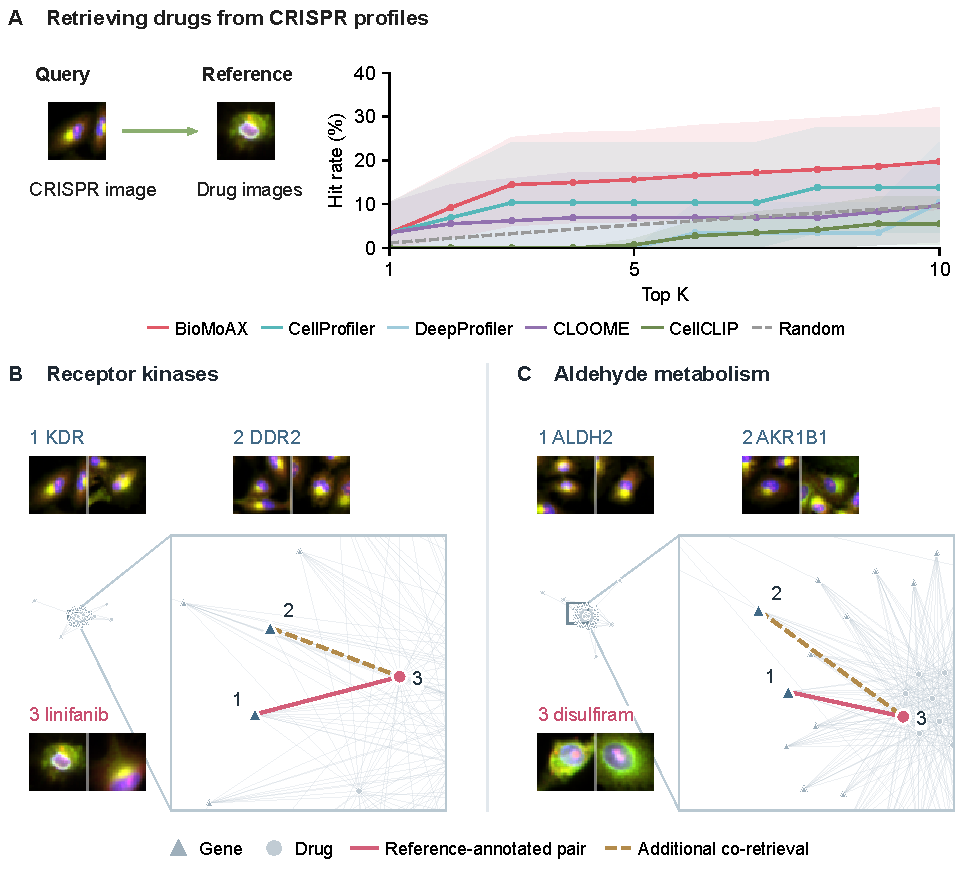
\includegraphics[width=\linewidth]{figures/fig5.pdf}
\caption{\csname captionFigure5\endcsname}\label{fig:5}
\end{figure}

Across 29 eligible gene queries and 1,038 reference drugs, BioMoAX achieved a Top-10 hit rate of 19.77\%, compared with 13.79\% for CellProfiler, the strongest baseline at this depth (Fig.~5A). This result extends the preceding drug-to-drug functional retrieval to genetic perturbations, connecting morphological responses of genes unseen during training to the drug reference library.

Perturbations of the receptor tyrosine kinases KDR and DDR2 both retrieved linifanib (Fig.~5B). KDR--linifanib is reference-annotated, with biochemical and cellular evidence supporting inhibition~\cite{albert2006}. An independent kinase screen also reported linifanib binding to DDR2, although this pair is absent from the current reference annotations~\cite{karaman2008}. Co-retrieval thus recovered an experimentally supported pharmacological relationship beyond the reference annotations, demonstrating how the shared representation can complement incomplete annotation.

The second example involves the aldehyde-metabolism genes ALDH2 and AKR1B1, which participate in oxidative and reductive metabolism of reactive aldehydes, respectively~\cite{chen2008aldh2,srivastava1998hne}. Both retrieved disulfiram (Fig.~5C). Experimental studies support inhibition of ALDH2 by disulfiram and its metabolites~\cite{lam1997disulfiram}; another study observed decreased AKR1B1 protein levels after disulfiram treatment in renal carcinoma xenografts~\cite{yoshino2020npl4}.

The two cases involve receptor tyrosine kinases and aldehyde-metabolism genes, respectively, illustrating the use of a shared drug as a phenotypic reference. Each case links a reference-annotated gene--drug pair to a second gene--drug association absent from the current reference annotations; independently reported drug binding or post-treatment protein changes provide biological support for these relationships. The shared space can therefore use existing drug responses to bring functionally related genetic perturbations into a common comparison framework, extending functional comparisons beyond current annotations.
